\section{SİMÜLASYON ÇALIŞMALARI}


\subsection{Simulasyon Yazılımları}

Simulasyonda verilerin elde edilmesi Python yazılımı üzerinden ve verilerin işlenmesi ise MATLAB yazılımı üzerinden yapılmıştır.

\subsubsection{Verilerin Elde Edilmesi}


\textbf{Yazılımda Kullanılan Kütüphaneler}

\begin{itemize}
    \item \textbf{serial:} Seri port üzerinden haberleşme sağlayarak MSP430 mikrodenetleyicisinden gelen verileri almak için kullanılıyor.
    \item \textbf{csv:} Toplanan verileri CSV dosyasına kaydetmek için kullanılıyor.
    \item \textbf{numpy:} Matematiksel hesaplamalar için kullanılıyor.
    \item \textbf{pandas:} CSV dosyasına veri yazmak için kullanılıyor.
    \item \textbf{pyqtgraph:} MSP430'dan gelen verilerin gerçek zamanlı grafiğini çizmek için kullanılıyor.
\end{itemize}

\textbf{Yazılımın Genel İşleyişi}

Yazılım, PyQtGraph kütüphanesi kullanarak bir grafiksel kullanıcı arayüzü (GUI) oluşturur. Bu GUI'da MSP430'dan gelen seri veri akışı LDR1 ve LDR2 için hem filtrelenmemiş hem de EMA yöntemi ile filtrelenmiş olarak sırasıyla ilk 2 çizelgede gösterilir. Son çizelgede ise bu LDR1 ve LDR2 içinde geri yönde sonlu fark gösterilir. Bu sonlu fark LDR'lerin önüne geçtiğinde negatif olur ve önünden çıktığında pozitif olur. Bu negatif ve pozitif değerleri kullanarak hareketin başlangıcı ve bitişi algılanır. Sonrasında veri sabit 500 örnek olması için eğer az veri alındıysa verideki maksimum değer eklenir ya da fazla veri alındıysa eşit aralıklarda bazı veriler çıkarılır ve istenen 500 örneğe ulaşılır. Bunu yapmamızın sebebi yapay zekanın sabit bir uzunlukta veri alması gerekmesidir.

\subsubsection{Verilerin İşlenmesi ve Yapay Zekanın Eğitilmesi}

Verilerin işlenmesi ve yapay zekada eğitilmesi bir MATLAB kodu ile yapılmıştır. Yazılım, önceden kaydedilen CSV dosyalarını okuyarak LDR1 ve LDR2’ye ait her biri 500 ölçüm içeren voltaj verilerini alır ve bu verileri tek bir vektörde birleştirerek 1000 ölçüm uzunluğunda bir vektör oluşturur. Kategorisel ("engin", "taha", "idris") bir veri seti oluşturulur. Bu veri seti için bir eğitim-doğrulama ayrım oranı belirlenir ve bu orana göre eğitim ve doğrulama alt kümeleri oluşturulur. Eğitim veri seti veri setinin ortalama sinyal gücünün belirli oranlarında gürültü eklenerek modelin girdisi oluşturulur ve çıktısı orijinal veridir. Bunun sebebi modelin eklenen gürültüler sayesinde genelleme yeteneğini arttırmak. Veri seti hazırlandıktan sonra Konvolüsyonel Gürültü Giderici Otokodlayıcı (CDAE) modeli, oluşturulan veri kümesi üzerinde eğitilir.

\subsection{Sistem Modelleme}

Sistem, LDR'ler üzerinden hareket tespiti yapmak için kullanılan verilerin toplanması, işlenmesi ve yapay zeka ile analiz edilmesi sürecini kapsamaktadır. Bu süreç, Python Yazılımı ve MATLAB Yazılımı olmak üzere iki ana aşamaya ayrılmıştır ve sistem diyagramında aşağıdaki gibi gösterilmiştir.

\subsubsection{Sistem Genel Görünümü}

\begin{itemize}
    \item \textbf{MSP430 Veri Toplama:} Sistem, MSP430 mikrodenetleyicisinden LDR1 ve LDR2'den gelen gerilim verilerinin 16-Bit ADC kullanılarak dijital değerlere çevrilmiş halini Bluetooth yoluyla alır.
    \item \textbf{Python Yazılımı (Veri Görselleştirme ve Kaydetme):}
    \begin{itemize}
        \item \textbf{Ham ADC Değerlerinin Voltaja Dönüştürülmesi:} Ham 12 bitlik ADC değerleri (ch0\_raw, ch1\_raw) 4 bit sola kaydırılarak oluşturulan 16 bitlik veriler, referans voltajı (REF\_VOLTAGE = 3.3 V) ve 16 bitlik bir tam sayının maksimum değeri (UINT16\_MAX = 65535) kullanılarak voltaja ölçeklenir. Denklemi şu şekildedir: ch0\_voltage = (ch0\_raw / UINT16\_MAX) * REF\_VOLTAGE.
        
        \item \textbf{EMA ile Veri Filtreleme:} Veriler bu yöntem kullanılarak filtrelenir. Bu yöntem, verilerdeki ani dalgalanmaları düzeltir ve önemli değişiklikleri tespit etmeyi kolaylaştırır. Filtrenin matematiksel denklemi şu şekildedir:
        
        \begin{equation}
            Y_t=\alpha X_t + (1-\alpha)Y_{t-1}
            \label{eq:ema}
        \end{equation}
        
        \eqref{eq:ema} de, \(\alpha\) filtreleme katsayısı 0.05 seçilmiştir, \(X_t\) şimdiki veri noktası, \(Y_t\) şimdiki filtrelenmiş veri noktası, \(Y_{t-1}\) bir önceki filtrelenmiş veri noktasıdır.

        \item \textbf{PyQtGraph ile Gerçek Zamanlı Grafikleme:} PyQtGraph ile Gerçek Zamanlı Grafikleme: Python yazılımı, PyQtGraph kütüphanesini kullanarak bir GUI oluşturur ve gelen verilerin voltajlarını ve sonlu farklarını gerçek zamanlı olarak çizer.

        \item \textbf{Geri Yönde Sonlu Fark ile Hareket Tespiti:} Sonlu fark yaklaşımı kullanılarak hareket tespiti yapılır. Bir nesne (örneğin bir kişi) LDR'lerin önünden geçtiğinde sonlu fark değeri negatif olur. Nesne uzaklaştığında ise bu değer pozitif olur. Bu işaret değişikliği, hareketin başlangıcı ve bitişini tespit etmek için kullanılır. Matematiksel denklemi şu şekildedir:

        \begin{equation}
            \nabla_h[V](t) = V_{t-1} - V_{t-1-h}
            \label{eq:finite_diff}
        \end{equation}
        
        \eqref{eq:finite_diff} de \(h\)'ın değeri 100'dür.
        
        \item \textbf{Veri Kaydetme:} Hareket tespiti sonuçları CSV formatında kaydedilir.
    \end{itemize}
    \item \textbf{MATLAB Yazılımı (Veri İşleme ve Yapay Zeka Eğitimi):}
    \begin{itemize}
        \item \textbf{Veri Eğitim/Doğrulama Ayırma:} Veriler belirli bir oranda eğitim ve doğrulama veri kümelerine ayrılır. Bu veri setleri, yapay zekayı eğitmek için kullanılır.

        \item \textbf{}
        
        \item \textbf{DNN Eğitimi:} Bu veri kümesi üzerinde Geri Yayılım yöntemi kullanılarak bir DNN eğitilir.
        
        \item \textbf{Simülasyon Tamamlanması:} Eğitim tamamlandıktan sonra, modelin performansı değerlendirilir ve sistem simülasyonu tamamlanır.
    \end{itemize}
\end{itemize}



\subsection{Simulasyonun Gerçekleştirilmesi}

Simülasyon, verilerin toplanması ve bu verilerle yapay zekanın eğitilmesi olmak üzere iki aşamaya ayrılabilir.


\subsubsection{Verilerin Toplanması}

İlk olarak, MSP430 mikrodenetleyicisi Bluetooth aracılığıyla bilgisayara bağlanır. Bağlantı kurulduktan sonra, hareketin başlangıç ve bitiş noktalarını belirlemek amacıyla geri yönde sonlu fark yöntemi kullanan bir Python kodu çalıştırılır. Ardından, bir kişi LDR'lerin önünden defalarca geçerek veri toplama işlemi gerçekleştirilir. Toplanan veriler CSV formatında kaydedilir. Bu süreci açıklayan bir UML diyagramı \ref{fig:simulasyongerçekleştirmesi}de görülmektedir.


\begin{figure}[H]
    \centering
    \includegraphics[width=\linewidth, keepaspectratio]{image3.png}
    \caption{Simulasyon Diyagramı}
    \label{fig:simulasyongerçekleştirmesi}
\end{figure}


\ref{fig:örnekverialımı_combined}de, cihazın ve bir kişinin hareketini ve bu hareketle alınan verilerin grafiği görülmektedir.


\subsubsection{Yapay Zekanın Eğitilmesi}

Toplanan veriler MATLAB’e yüklenir. Elde edilen veri kümesi, eğitim ve doğrulama olarak ikiye ayrılır. CDAE katmanları ve eğitim seçenekleri belirlenir. Son olarak yapay zeka modeli eğitilir. CDAE mimarisi ise \ref{fig:model_temsili}de temsili olarak sunulmaktadır. CDAE mimarisinde, çok sayıda nöron bulunduğundan, görsel bütünlüğün korunabilmesi amacıyla saklı katmanlardaki her bir nöron çizilmemiştir.

\begin{figure}[H]
    \centering
    \includegraphics[width=\linewidth]{media/model_temsili.jpg}
    \caption{Modelimizin temsili mimarisi}
    \label{fig:model_temsili}
\end{figure}

\begin{figure}[H]
    \centering
    \begin{subfigure}[t]{0.49\textwidth} % Adjust the width to less than 0.5\textwidth
        \centering
        \includegraphics[width=\linewidth]{image23}
    \end{subfigure}
    \hfill % Adds horizontal space between the figures
    \begin{subfigure}[t]{0.49\textwidth} % Adjust the width to less than 0.5\textwidth
        \centering
        \includegraphics[width=\linewidth]{plot2}
    \end{subfigure}
    \caption{MSP430 ADC Verileriyle Algılanan Bir Kişinin Geçişine Ait Veriler ve Grafiği}
    \label{fig:örnekverialımı_combined}
\end{figure}




\begin{comment}

\begin{figure}[H]
    \centering
    %%\drawNN{8, 25, 50, 25, 3}{Girdi Katmanı, Saklı \\ Katman 1, Saklı \\ Katman 2, Saklı \\ Katman 3, Çıktı Katmanı}{LDR 2 Minimum, LDR 2 Maksimum, LDR 2 RMS, LDR 2 Ortalama, LDR 1 Minimum, LDR 1 Maksimum, LDR 1 RMS, LDR 1 Ortalama}{2.5}{0.75}{11}
    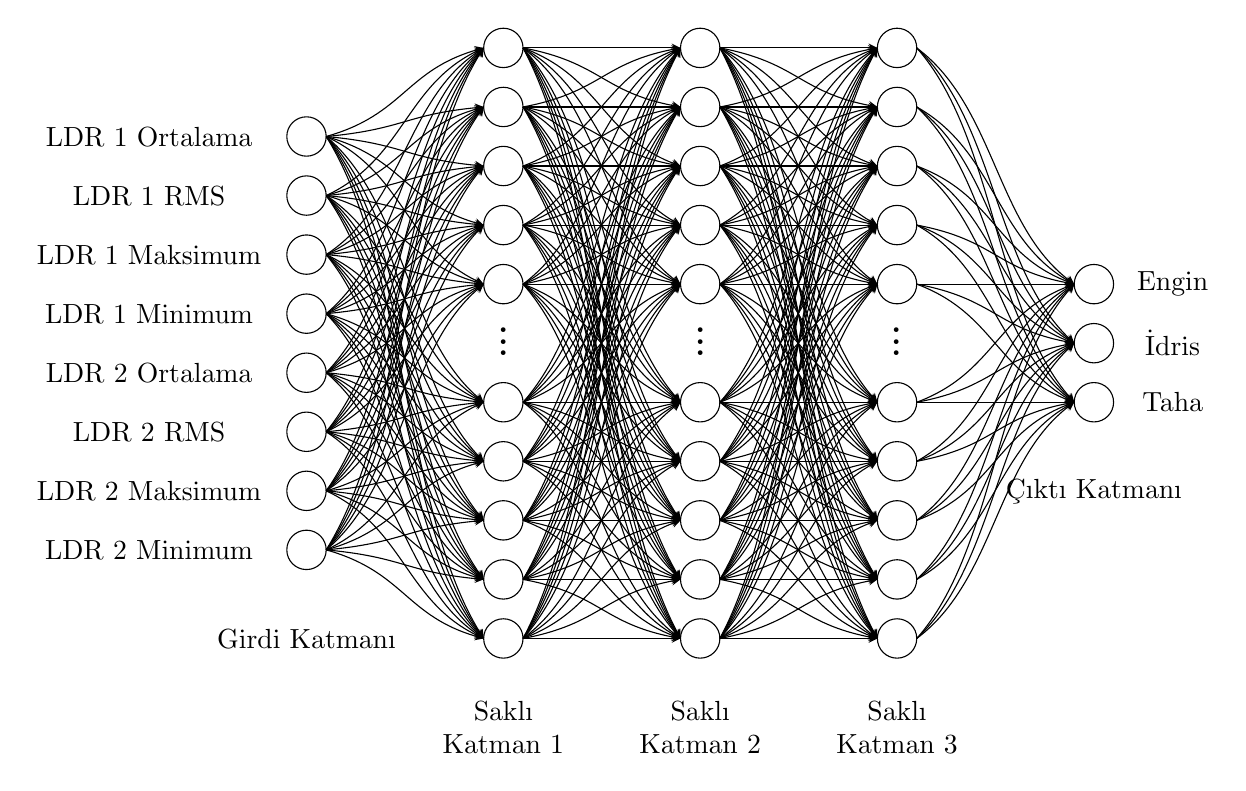
\begin{tikzpicture}[
    neuron/.style={circle, draw, minimum size=0.5cm, inner sep=0},
    arrow/.style={->, thick},
    align=center
    ]


    % Base coordinates
    \def\layers{8, 25, 50, 25, 3} % Example: 3 input, 4 hidden, 3 hidden, 1 output
    \def\labels{Girdi Katmanı, Saklı \\ Katman 1, Saklı \\ Katman 2, Saklı \\ Katman 3, Çıktı Katmanı}
    \def\features{LDR 2 Minimum, LDR 2 Maksimum, LDR 2 RMS, LDR 2 Ortalama, LDR 1 Minimum, LDR 1 Maksimum, LDR 1 RMS, LDR 1 Ortalama}
    \def\outputs{Taha, İdris, Engin}
    \def\xstart{0}    % X-coordinate for the first layer
    \def\layersep{2.5}  % Horizontal separation between layers
    \def\ysep{0.75}    % Vertical separation between neurons
    \def\maxneuron{11} % Threshold for number of neurons to display
    \pgfmathsetmacro{\mn}{int((\maxneuron-1)/2)}
    \pgfmathsetmacro{\ys}{int((\maxneuron+1)/2)}
    
    
    
    \foreach \i [count=\n from 1] in \layers {
        \ifnum\n = 1
            \foreach \feature [count=\n from 1] in \features {
                \pgfmathsetmacro{\yshift}{- (\i + 1) * \ysep / 2}
                \node[] at (-2, \yshift + \n*\ysep) {\feature};
            }
        \fi
    }

    \foreach \i [count=\n from 1] in \layers {
        \ifnum\n = 1
            \foreach \out [count=\n from 1] in \outputs {
                \pgfmathsetmacro{\yshift}{- (3 + 1) * \ysep / 2}
                \node[] at (1 + 4*\layersep, \yshift + \n*\ysep) {\out};
            }
        \fi
    }

    
    
    
    % Process layers and neurons
    \foreach \i [count=\n from 1] in \layers {
        % Calculate the x-coordinate for the layer
        \pgfmathsetmacro{\xpos}{\xstart + (\n-1)*\layersep}
        
        % Draw neurons for the current layer and store node names in a list
        \ifnum\i > \maxneuron
            % Calculate vertical starting position for the neurons
            \pgfmathsetmacro{\yshift}{-\ys*\ysep}
            
            % Draw four neurons for the current layer
            \foreach \m in {1,2,...,\mn} {
                \pgfmathsetmacro{\t}{int(\maxneuron-\m)}
                \node[neuron] (L\n N\m) at (\xpos, \yshift + \m*\ysep) {};  % Node name L<layer> N<neuron>
                \node[neuron] (L\n N\t) at (\xpos, \m*\ysep) {};
            }
            % Add vertical ellipsis between second and third neuron
            \node at (\xpos, 0.125) {\huge$\vdots$};
        \else
            % Calculate vertical starting position for the neurons
            \pgfmathsetmacro{\yshift}{- (\i + 1) * \ysep / 2}
            
            
            % Draw all neurons for the current layer
            \foreach \m in {1,...,\i} {
                \node[neuron] (L\n N\m) at (\xpos, \yshift + \m*\ysep) {};  % Node name L<layer> N<neuron>
            }
        \fi
    }
    
    
    % Add layer labels
    \foreach \a [count=\m from 1] in \layers {
        \foreach \label [count=\n from 1] in \labels {
            \ifnum\n= \m
                \pgfmathsetmacro{\xpos}{(\n-1)*\layersep}
                \ifnum\a > \maxneuron
                    % Calculate vertical starting position for the neurons
                    \pgfmathsetmacro{\yshift}{-\maxneuron*\ysep/2}
                \else
                    % Calculate vertical starting position for the neurons
                    \pgfmathsetmacro{\yshift}{-\a*\ysep/2}
                \fi
                \node[align=center, font=\rmfamily] at (\xpos, \yshift - \ysep) {\label};
            \fi
        }
    }


    
    
    % Loop through the list using pgffor
    \foreach \i [count=\n] in \layers {
        \foreach \j [count=\m] in \layers {
            \ifnum\m=\numexpr\n+1\relax
                \ifnum\i > \maxneuron
                    \pgfmathsetmacro{\ie}{\maxneuron-1}
                    \ifnum\j > \maxneuron
                        \pgfmathsetmacro{\je}{\maxneuron-1}
                        \foreach \k in {0,...,\ie} {
                            \foreach \p in {0,...,\je} {
                                \ifnum \numexpr2*\k = \ie 
                                \else
                                    \ifnum \numexpr2*\p = \je 
                                    \else
                                    \pgfmathsetmacro{\xpos}{\xstart + (\n-1)*\layersep}
                                    \pgfmathsetmacro{\yshift}{-\ys*\ysep}
                                    
                                    \pgfmathsetmacro{\nextlayer}{int(\n+1)}
                                    \draw[->, >=stealth] (\xpos + 0.25, \yshift + \k*\ysep + \ysep) .. controls (\xpos + \layersep / 2, \yshift + 3*\k*\ysep/4 + \p * \ysep / 4 + \ysep) and (\xpos + \layersep / 2, \yshift + 3*\p*\ysep / 4 + \k * \ysep / 4 + \ysep) .. (\xpos - 0.25 + \layersep, \yshift + \p*\ysep + \ysep);
                                    \fi
                                \fi
                            }
                        }
                    \else
                        \pgfmathsetmacro{\je}{\j}
                        \foreach \k in {0,...,\ie} {
                            \foreach \p in {1,...,\je} {
                                \ifnum \numexpr2*\k = \ie 
                                \else
                                \pgfmathsetmacro{\xpos}{\xstart + (\n-1)*\layersep}
                                \pgfmathsetmacro{\yshiftl}{- \ys * \ysep}
                                \pgfmathsetmacro{\yshiftr}{- (\je+1) * \ysep / 2}
                                
                                
                                \pgfmathsetmacro{\nextlayer}{int(\n+1)}
                                \draw[->, >=stealth] (\xpos + 0.25, \yshiftl + \k*\ysep + \ysep) .. controls (\xpos + \layersep / 2, 3*\yshiftl/4 + 3*\k*\ysep/4 + 3*\ysep/4 + \yshiftr/4 + \p*\ysep/4) and (\xpos + \layersep / 2, 3*\yshiftr/4 + 3*\p*\ysep/4 + \yshiftl/4 + \k*\ysep/4 + \ysep / 4) .. (\xpos - 0.25 + \layersep, \yshiftr + \p*\ysep);
                                \fi
                            }
                        }
                    \fi
                \else
                    \pgfmathsetmacro{\ie}{\i}
                    \ifnum\j > \maxneuron
                        \pgfmathsetmacro{\je}{\maxneuron-1}
                        \foreach \k in {1,...,\ie} {
                            \foreach \p in {0,...,\je} {
                                \ifnum \numexpr2*\p = \je 
                                \else
                                \pgfmathsetmacro{\xpos}{\xstart + (\n-1)*\layersep}
                                \pgfmathsetmacro{\yshiftl}{- (\ie + 1) * \ysep / 2}
                                \pgfmathsetmacro{\yshiftr}{-\ys * \ysep}
                                
                                
                                \pgfmathsetmacro{\nextlayer}{int(\n+1)}
                                \draw[->, >=stealth] (\xpos + 0.25, \yshiftl + \k*\ysep) .. controls (\xpos + \layersep / 2, 3*\yshiftl/4 + 3*\k*\ysep/4 + \yshiftr/4 + \p*\ysep/4 + \ysep/4) and (\xpos + \layersep / 2, 3*\yshiftr/4 + 3*\p*\ysep/4 + 3*\ysep/4 + \yshiftl/4 + \k*\ysep/4) .. (\xpos - 0.25 + \layersep, \yshiftr + \p*\ysep + \ysep);
                                \fi
                            }
                        }
                    \else
                        \pgfmathsetmacro{\je}{\j}
                        \foreach \k in {1,...,\ie} {
                            \foreach \p in {1,...,\je} {
                                \pgfmathsetmacro{\xpos}{\xstart + (\n-1)*\layersep}
                                \pgfmathsetmacro{\yshiftl}{- (\ie + 1) * \ysep / 2}
                                \pgfmathsetmacro{\yshiftr}{- (\je + 1) * \ysep / 2}
                                
                                \pgfmathsetmacro{\nextlayer}{int(\n+1)}
                                \draw[->, >=stealth] (\xpos + 0.25, \yshiftl + \k*\ysep) .. controls (\xpos + \layersep / 2, 3*\yshiftl/4 + 3*\k*\ysep/4 + \yshiftr/4 + \p*\ysep/4) and (\xpos + \layersep / 2, 3*\yshiftr/4 + 3*\p*\ysep/4 + \yshiftl/4 + \k*\ysep/4) .. (\xpos - 0.25 + \layersep, \yshiftr + \p*\ysep);
                            }
                        }
                    \fi
                \fi
            \fi
        }
    }
    
    
    \end{tikzpicture}
    \caption{DNN Mimarisi}
    \label{fig:yapayzekamimarisi}
\end{figure}

\end{comment}





\begin{comment}
Her çalışmanın mutlaka bir simülasyonu yapılmalıdır. Simülasyon
çalışmaları Tasarım Projesi kapsamında yapılabilecek kısımdır.
Simülasyon yazılımı, çalışmayı yapan öğrenciler tarafından
geliştirilebileceği gibi paket programlar da kullanılabilir. Simülasyon
çalışmasında kullanılacak modellenmenin nasıl yapıldığı açıklanmalı ve
matematiksel model denklemleri önceki bölümlerde yapılan çalışmalara da
dayanılarak verilmelidir. Hazır paket program kullanılıyorsa çalışmanın
bu paket programda nasıl kullanıldığı, bu paket program için nasıl
modellendiği, hangi veriler kullanılarak simülasyon yapıldığı
açıklanmalıdır. Simülasyon sonuçları \emph{Sonuçlar} bölümünde
verilmelidir.

Bu bölümde kullanılabilecek muhtemel alt başlıklar aşağıdaki gibi
olabilir.

\textbf{4.2. Simülasyon Yazılımı}

Çalışma kapsamında geliştirilen veya hazır kullanılacak olan simülasyon
yazılımı hakkında bilgiler verilir. Yazılım kısaca tanıtılır ve bu
çalışmada nasıl kullanılacağı açıklanır.

\textbf{4.2. Sistem Modelleme}

Simülasyonu yapılacak olan sistemin nasıl modellendiği açıklanır ve
model denklemleri ya da model şekli verilir. Gerekli açıklamalar
yapılır, modelin nasıl çalıştığı anlatılır.

\textbf{4.3. Simülasyon}

Simülasyon diyagramları ve simülasyonun nasıl gerçekleştirildiği bu
ayrıtta açıklanır.

\end{comment}

\begin{comment}
\textbf{5. DENEYSEL ÇALIŞMALAR}

\textbf{(Bu bölüm Mühendisli Tasarımı Projesinde yoktur.)}

\textbf{5.1. Genel Bilgiler}

Deneysel Çalışmalar, bu başlık altında verilir. Tasarım Projesi bu kısmı
içermediğinden, Tasarım Projesi Sonuç Raporu da bu bölümü içermez. Bu
bölüm Bitirme Projesi Kitabında yer alır.

Kurulan düzeneğinin ya da gerçekleştirilen pratik çalışmanın nasıl
gerçekleştirildiği bu bölümde açıklanmalıdır. Bu gerçekleştirme
sırasında yaşanan zorluk ve kolaylıkların neler olduğu, pratik
çalışmanın nasıl çalıştığı, bunu başkasının nasıl kullanabileceği
bilgileri verilmelidir. Pratik çalışmada standartlar dâhilinde hangi
güvenlik önlemlerinin alındığı belirtilmelidir. Çalışma üzerinde
kullanımda gerekli tüm işaretlendirmeler yapılmalı, varsa uyarılar
konulmalıdır. Bu işaretleme ve uyarılar pratik çalışmanın üzerinde
mutlaka olmalı, ayrıca bitirme kitapçığının bu bölümünde de yer
almalıdır. Fazla güvenlik uyarısı varsa ayrı bir bölüm olarak da
düzenlenebilir. Bu bölümde \textbf{pratik çalışmanın bağlantı şemaları,
baskı devre çizimleri ve sistemin fotoğrafları verilmelidir. Anlaşılır
bağlantı diyagramı mutlaka çizilerek konmalıdır. Fotograf bağlantı
diyagramı değildir.}

Genel Bilgiler alt başlığında, bu bölümde nelerden bahsedileceği kısaca
anlatıldıktan sonra ayrıntılara geçilir. Ayrıntılar devam eden alt
başlıklar altında anlatılır. Örneğin daha önce Bölüm 2. de kullanılan
Rüzgar Enerji Sistemi örneği ele alınırsa diğer alt başlıklar aşağıdaki
gibi olabilir.

\textbf{5.2. Rüzgar Türbini ve Generatör Sisteminin Birleştirilmesi}

Çalışmada kullanılan rüzgar türbini ve generatör kısaca tanıtıldıktan
sonra bunların nasıl birleştirildikleri açıklanır. Tanıtımları
yapılırken kullanılan türbin ve genetatörün teknik özellikleri
açıklanmalı ve bu çalışmada nasıl kullanıldıkları anlatılmalıdır. Ayrı
ayrı ve/veya birleştirilmiş hallerinin fotoğrafı da kullanılabilir.
Ancak doğru olanı, teknik çizimle birleşim şemasının tasarımın
anlatıldığı 3. Bölümde verilmiş olmasıdır. Bu alt başlığın içeriği proje
konu ve kapsamına göre düzenlenmelidir. Burada verilen konu sadece
örnektir.

\textbf{5.3. Arayüz Elemanlarının Gerçeklenmesi}

Çalışmadaki farklı sistemlerin birleştirilmesinde kullanılan arayüz
elemanları ve nasıl kullanıldıkları, pratik olarak nasıl
gerçekleştirildikleri bu ayrıtta açıklanmalıdır. Çalışmanın konusu ve
kapsamına göre başlığın adı değişebilir. Örnek olarak verilen Rüzgar
Enerji Sistemleri ile ilgili çalışmada generatörün şebeke veya yüklere
bağlantısını sağlayan ara güç elektroniği elemanlarının (Doğrultucu,
evirici, kıyıcı, vb.) nasıl gerçekleştirldikleri ve monte edildikleri bu
ayrıtta açıklanabilir. Gerekirse 5.3.1., 5.3.2. gibi yeni alt başlıklar
açılarak farklı ara elemanların gerçeklenmesi detaylı olarak
açıklanabilir. Örneğin yine Rüzgar Enerji Sistemi başlıklı çalışmayı ele
alırsak bu 2. Alt başlıklar aşağıdaki gibi olabilir.

5.3.1. Evirici ve Sürücü devreleri

5.3.2. Eviricinin Kontrolü

5.3.3. Yükler

Bu kısımda kullanılan ara elemanlardaki komponentlerden bahsederken
onların teknik özellikleri anlatılmalıdır. Örneğin kullanılan bir diyodu
anlatırken diyodun fotoğrafını koyup geçilmemeli, buı diyodun
karakteristik özellikleri, çalışma eğrisi üzerinden açıklanmalıdır.



\textbf{5.4. Yapılan Testler}

Tasarlanan sistemin gerçeklenmesi tamamlandıktan sonra üretim (yapım)
amacına uygun olarak çalışıp çalışmadığı test edilerek bu testlerin
nasıl yapıldığı bu ayrıtta açıklanmalıdır. Testlşerin hangi koşullar
altında hangi özel durumlar dikkate alınarak yapıldığı, yapılan kabuller
vb. Burada verilmelidir. Varsa test sisteminin bağlantı diyagramları
verilmeli ve açıklanmalıdır. Sonuçların listelenmesi, çizilmesi, ve
yorumlanması bu bölümde değil, bir sonraki bölümde verilmelidir.
\end{comment}

\begin{comment}
İşlemci değişti.

Uygunluk Kontrolü
4.1 Genel Bilgiler:
Yönerge simülasyonun zorunlu olduğunu, kullanılan yazılımın açıklanmasını ve matematiksel modelin verilmesini istiyor. Mevcut metinde Python ve MATLAB yazılımları açıklandı. Python’da kullanılan filtreleme ve sonlu fark formülleri matematiksel olarak verildi.
→ Uygun

4.2 Simülasyon Yazılımı:
Hem Python hem MATLAB yazılımları detaylandırılmış. Kütüphaneler, genel işleyiş, veri işleme ve eğitim aşamaları anlatılmış.
→ Uygun

4.3 Sistem Modelleme:
Sistem mimarisi, veri toplama, işleme ve model eğitimi aşamaları ayrıntılı anlatılmış. Matematiksel ifadeler ve modellemeye yönelik formüller (EMA ve sonlu fark) verilmiş.
→ Uygun

4.4 Simülasyonun Gerçekleştirilmesi:
Simülasyon adımları ayrıntılı ve diyagramlar görsel olarak desteklenmiş.
→ Uygun

Öneriler (İyileştirme İçin)
Başlık Uyumu:
Metin 1’de alt başlıklar şöyle verilmiş:

4.1 Genel Bilgiler

4.2 Simülasyon Yazılımı

4.3 Sistem Modelleme

4.4 Simülasyon (ya da Simülasyonun Gerçekleştirilmesi)

Sizde 4.1 başlığı "Simulasyon Yazılımları" olarak verilmiş. Yönergeyle uyum için 4.1 “Genel Bilgiler” ve 4.2 “Simülasyon Yazılımları” şeklinde bölünebilir.

Model Denklemlerinin Öne Çıkarılması:
EMA ve sonlu fark denklemleri güzel, fakat sistem modellemesinde özellikle yapay zekanın DNN yapısı matematiksel olarak da kısaca ifade edilebilir veya modelleme kısmında formül/denklem şeklinde açıklanabilir. (Örneğin, giriş ve çıkış verisi tanımları, kullanılan katman sayısı vb.)

Simülasyon Yazılımının Kullanımı:
MATLAB’ın nasıl kullanıldığı biraz daha ayrıntılı anlatılabilir. Örneğin, hangi fonksiyonlar veya toolbox kullanıldı, kullanıcı arayüzü var mı, parametre ayarları nasıl yapıldı vb.

Simülasyon Sonuçlarının Yerleşimi:
Yönergede simülasyon sonuçlarının “Sonuçlar” bölümünde verilmesi istenmiş. Mevcut metinde sonuçlar kısmı yok, bunun ayrı bir bölümde ele alınması uygun olur.



\end{comment}

